\subsection{ \textbf{$p_T$ smearing} }

为了让模拟的结果可以更好的反应探测器的分辨率带来的影响,在进行强子衰变模拟的时候需要对末态粒子的横动量相对于模拟的值添加一个小的增量。这个增量可以为正值也可以是负值。这个添加增量的过程被称作$p_T$ smearing。

在STAR官方的模拟(embedding)当中,已可以在一定程度上反应探测器对径迹动量的影响。但因为时间投影室当中可以影响到最后横动量测量结果的因素多且复杂,以及STAR的高亮度的测量环境本身也会对横动量的测量带来影响,这就使得embedding中的探测器的分辨率相比于真实情况更加的精确。即在相同动量下同一个粒子(如$J/\psi$)的谱的宽度会变得比测量结果更窄。这就需要调整$p_T$ smearing的参数使得模拟结果可以更好的描述数据。

首先需要确定描述得到探测器的分辨率的方法。在embedding的数据当中,可以得到$\delta_{p_T}/p_T ~v.s.~p_T$的二维分布。将数据分成多个不同的$p_T$区间,各个区间内在 $\delta_{p_T}/p_T$的峰值附近进行高斯拟合,得到的高斯拟合的宽度便可以确定在每个$p_T$区间内的探测器的分辨,如图\ref{fig:Pt_res}所示。
探测器的分辨$\sigma_{p_T}/p_T$随$p_T$变化的曲线,如图\ref{fig:pT_res_embd}所示。其中拟合曲线为式\ref{eq:pT_res}。当得到a的值之后,接下来要做的就是对在一定变化范围内对a的值进行扫描,从而对描述探测器分辨的方程进行标定,从而确定可以最好地描述数据的a的值。
\begin{figure}[htb]
    \centering
    \begin{subfigure}[b]{0.45\textwidth}
        \centering
        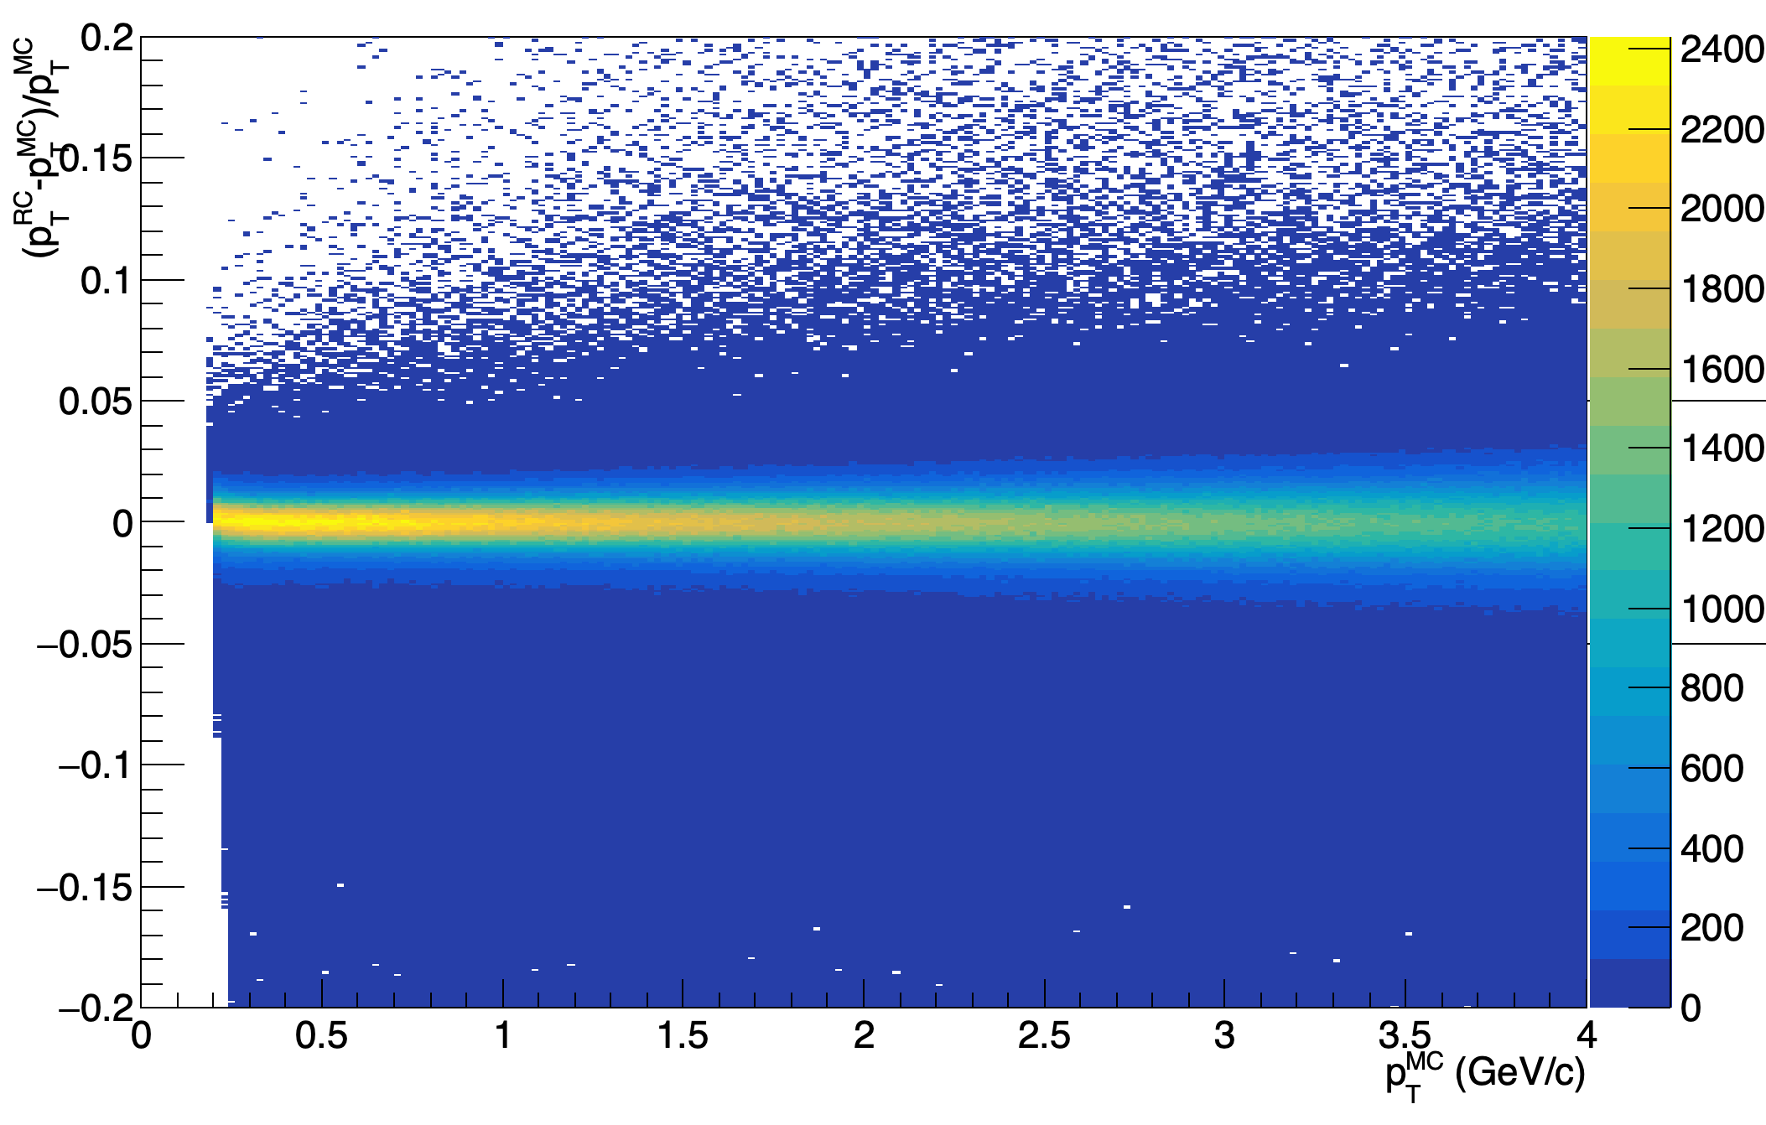
\includegraphics[width=\textwidth,clip]{figures/Chapter4/Pt_res_2D.png}
        \caption{}
        \label{fig:Pt_res_2D}
    \end{subfigure}
    \hfill
    \begin{subfigure}[b]{0.45\textwidth}
        \centering
        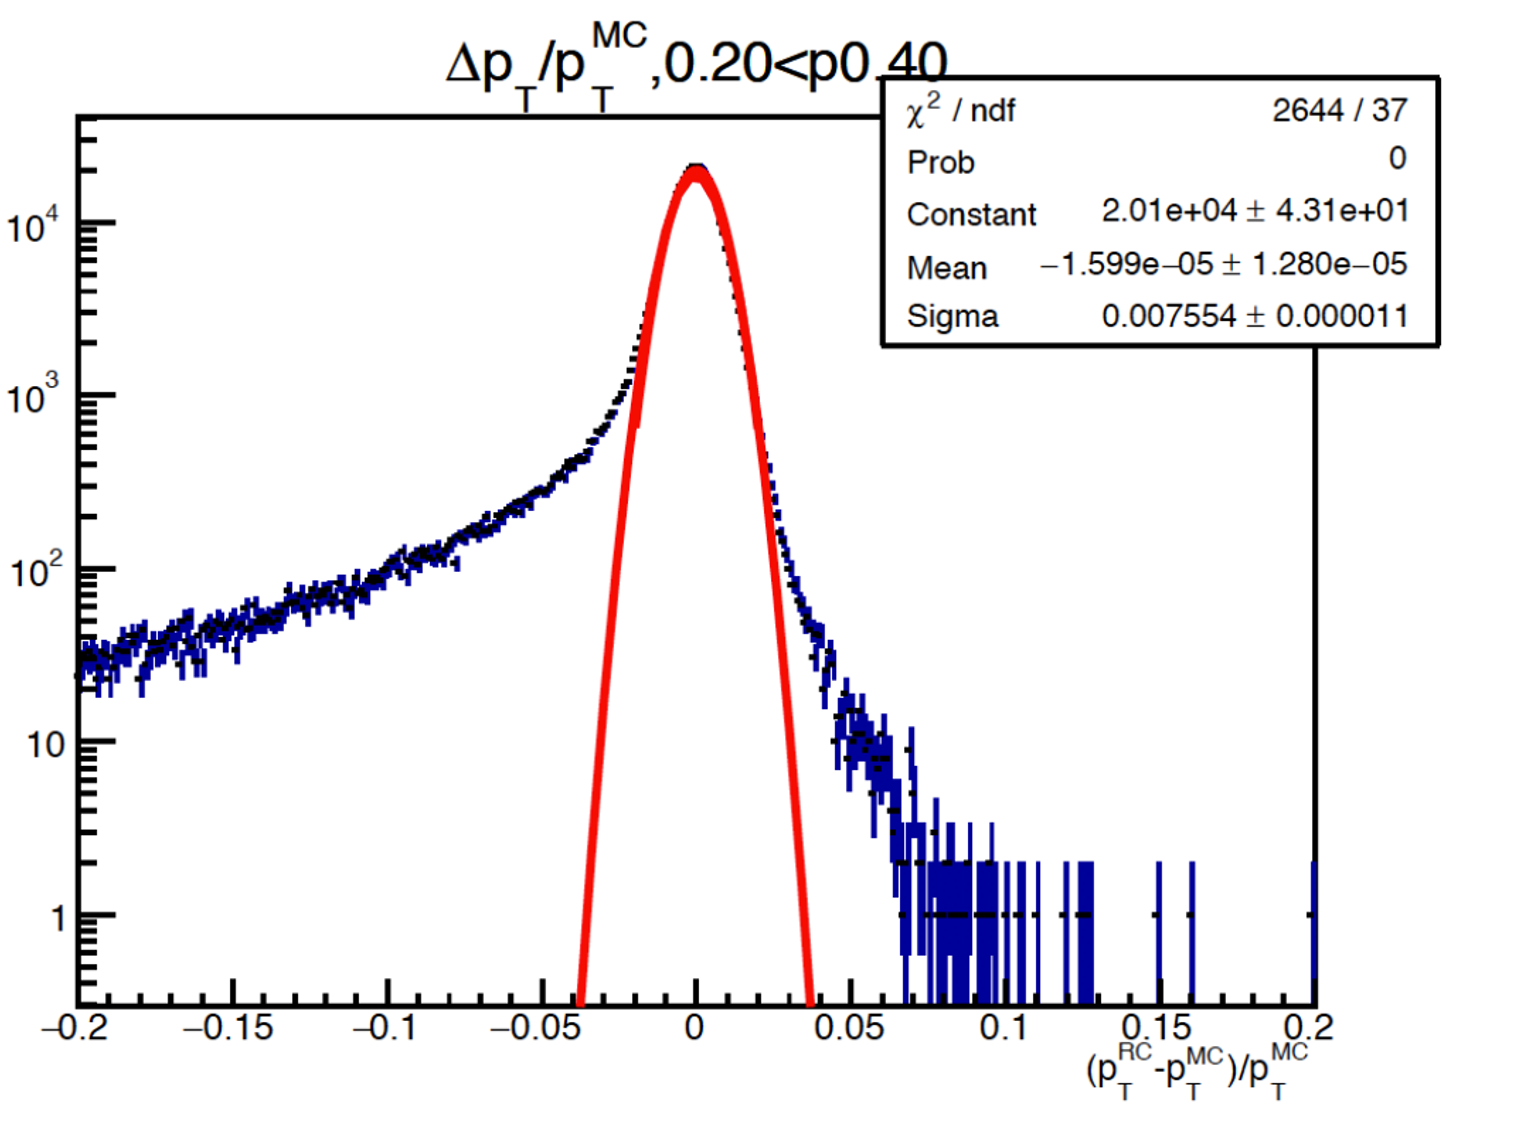
\includegraphics[width=\textwidth,clip]{figures/Chapter4/Pt_res_fit.png}
        \caption{}
        \label{fig:Pt_res_fit}
    \end{subfigure}
    \caption[0-80\%中心度下embedding 中的$\delta_{p_T}/p_T$分布示意图]{0-80\%中心度下embedding 中的$\delta_{p_T}/p_T$分布示意图,左图为$ \sigma_{p_T}/p_T~v.s.~p_T$的二维分布。右图为 $\rm{0.2 < p_T < 0.4~GeV/c}$ 区间内的拟合结果,拟合曲线为高斯函数。 }
    \label{fig:Pt_res}
\end{figure}
\begin{equation}
    \label{eq:pT_res}
    \delta_{p_T} = \sqrt{a^2 p_T^2 + b^2}
\end{equation}

\begin{figure}[htb]
    \begin{center}
    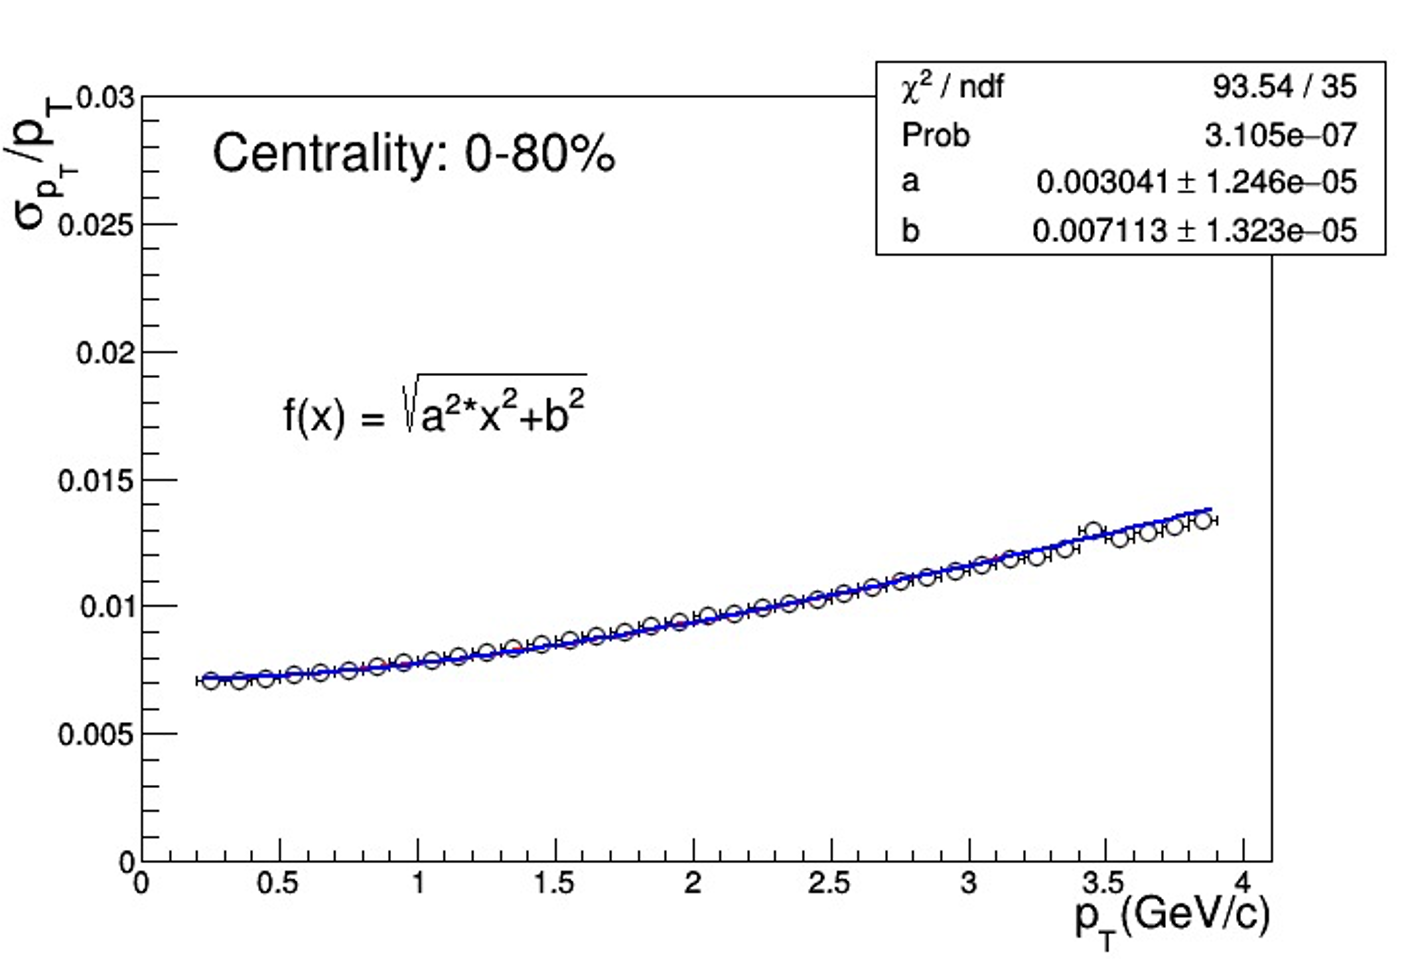
\includegraphics[width=0.8\textwidth,clip]{figures/Chapter4/pT_res_embd.png}
    \end{center}
    \caption[横动量分辨率随横动量变化示意图]{0-80\%中心度下横动量分辨率随横动量变化示意图,并通过拟合得到$\sigma_{p_T}/p_T$随$p_T$变化的曲线,拟合方程在图中标出。}
    \label{fig:pT_res_embd}
\end{figure}

因为$\rm{J/\psi}$有着信噪比高的优势,所以在本分析当中$\rm{J/\psi}$的信号被选取用来作为标定的参考信号。以0-80\%中心度为例,首先在0.001-0.021的范围内每隔0.0001取一个不同的a的值。这些不同的a的值分别作为$p_T$ smearing输入的参数产生$\rm{J/\psi}$的模拟结果。再用这些不同的模拟结果去拟合数据中的$\rm{J/\psi}$分布。使拟合的$\chi^2$最小的a的值就是可以最好地描述数据的a的值,在相同中心度下不同的物理过程模拟中均使用这个值作为$p_T$ smearing参数。a值扫描结果如图\ref{fig:Chi2_TuneA}所示。在不同中心度下的a的值见表\ref{tab:a}。
\begin{figure}[htb]
    \begin{center}
    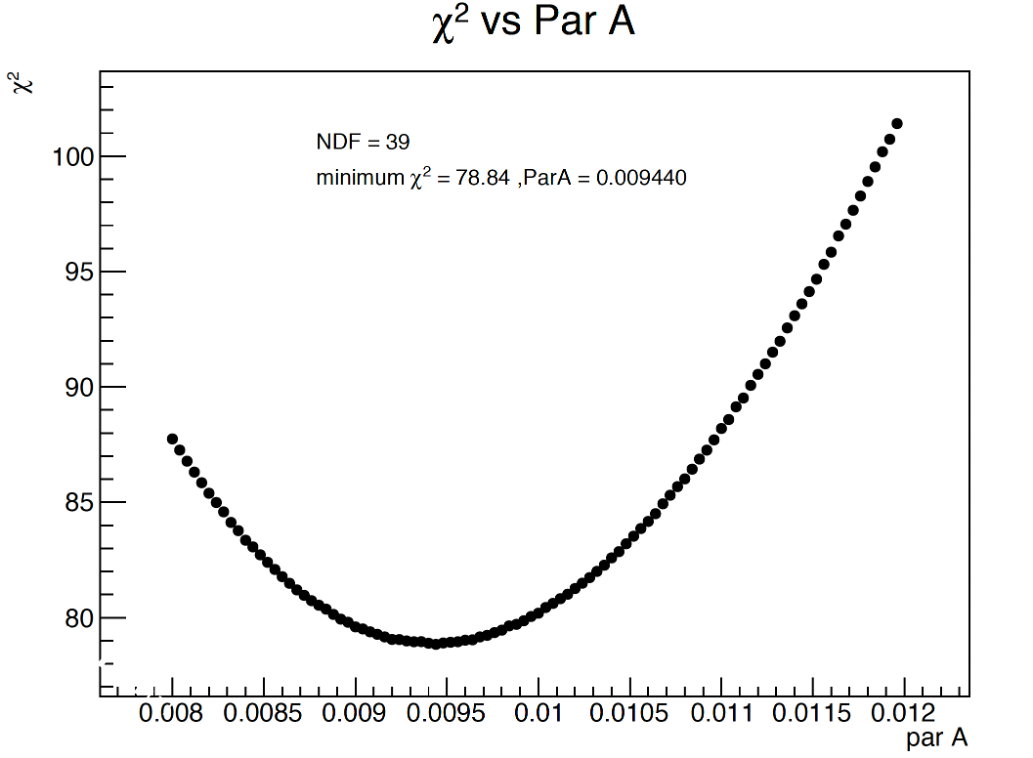
\includegraphics[width=0.8\textwidth,clip]{figures/Chapter4/Chi2_TuneA.png}
    \end{center}
    \caption[不同参数a时模拟样本拟合数据的$\chi^2$分布]{寻找最佳参数a时不同a下$\chi^2$的值}
    \label{fig:Chi2_TuneA}
\end{figure}
\begin{table}[h!]
    \centering
    \caption{\sNN = 54.4 GeV 金-金对撞中不同中心度下a的值}
    \label{tab:a}
    \begin{tabularx}{0.8\textwidth} {
    | >{\centering\arraybackslash}X  |>{\centering\arraybackslash}X | }
    \hline
    Centrality & a \\
    \hline
    0-80\% & 0.006450 \\
    \hline
    0-10\% & 0.005600 \\
    \hline
    10-40\% & 0.007700 \\
    \hline
    40-80\% & 0.008250 \\
    \hline
    \end{tabularx}
\end{table}